\newpage
\section{Análise transônica dos perfis}

Na condição de projeto ($M_n = 0{,}7196$, $c_\ell = 0{,}7319$)
comparamos o NACA~1411 reescalado com o otimizado da
Tabela~\ref{tab:airfoils_opt}: geometria, $C_p$ e Mach ao longo da
corda.

\begin{figure}[H]
    \centering
    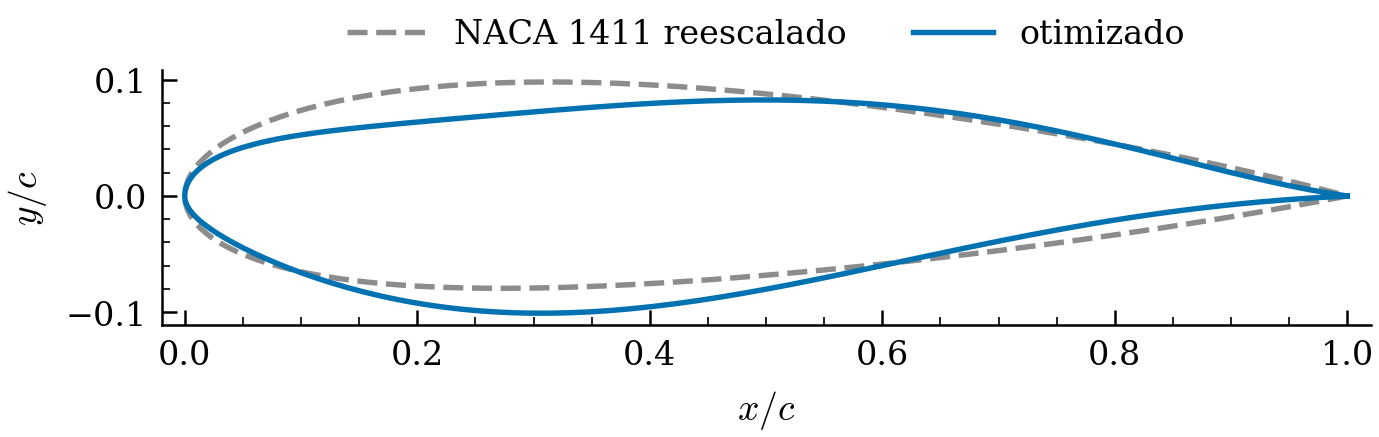
\includegraphics[width=0.8\textwidth]{images/05_transonico/geometria.png}
    \caption{Geometrias sobrepostas: a espessura máxima recua de
    $x/c = 0{,}296$ para $0{,}364$; o arqueamento máximo vai de
    $+0{,}010$ para $-0{,}015$.}\label{fig:geom_overlay}
\end{figure}

\begin{figure}[H]
    \centering
    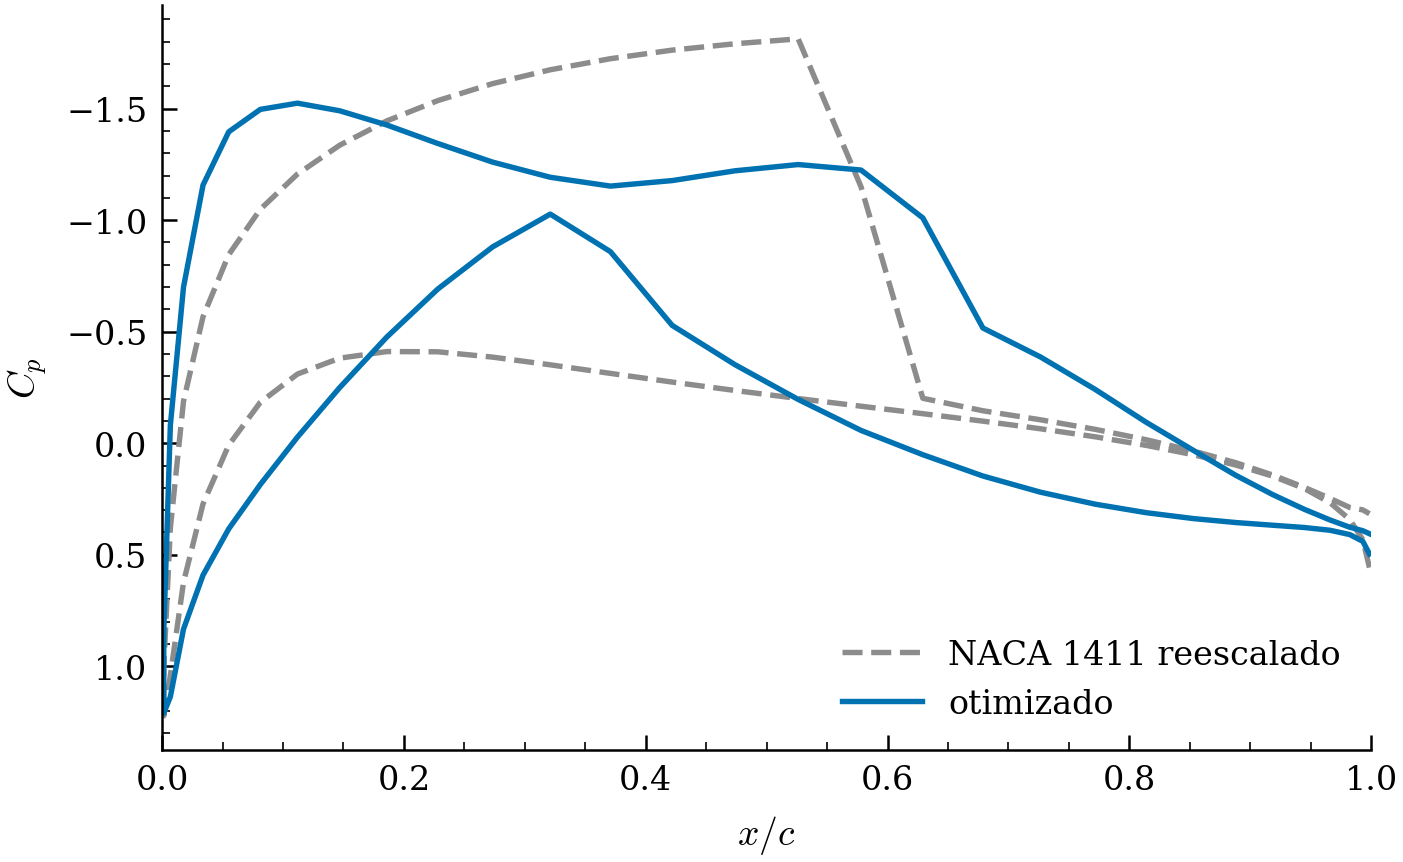
\includegraphics[width=0.8\textwidth]{images/05_transonico/cp.png}
    \caption{$C_p$ na condição de projeto: o NACA tem pico e degrau de
    choque em $x/c \approx 0{,}55$; o otimizado espalha a carga
    ($c_d = 0{,}06705 \to 0{,}01164$).}\label{fig:cp_overlay}
\end{figure}

\begin{figure}[H]
    \centering
    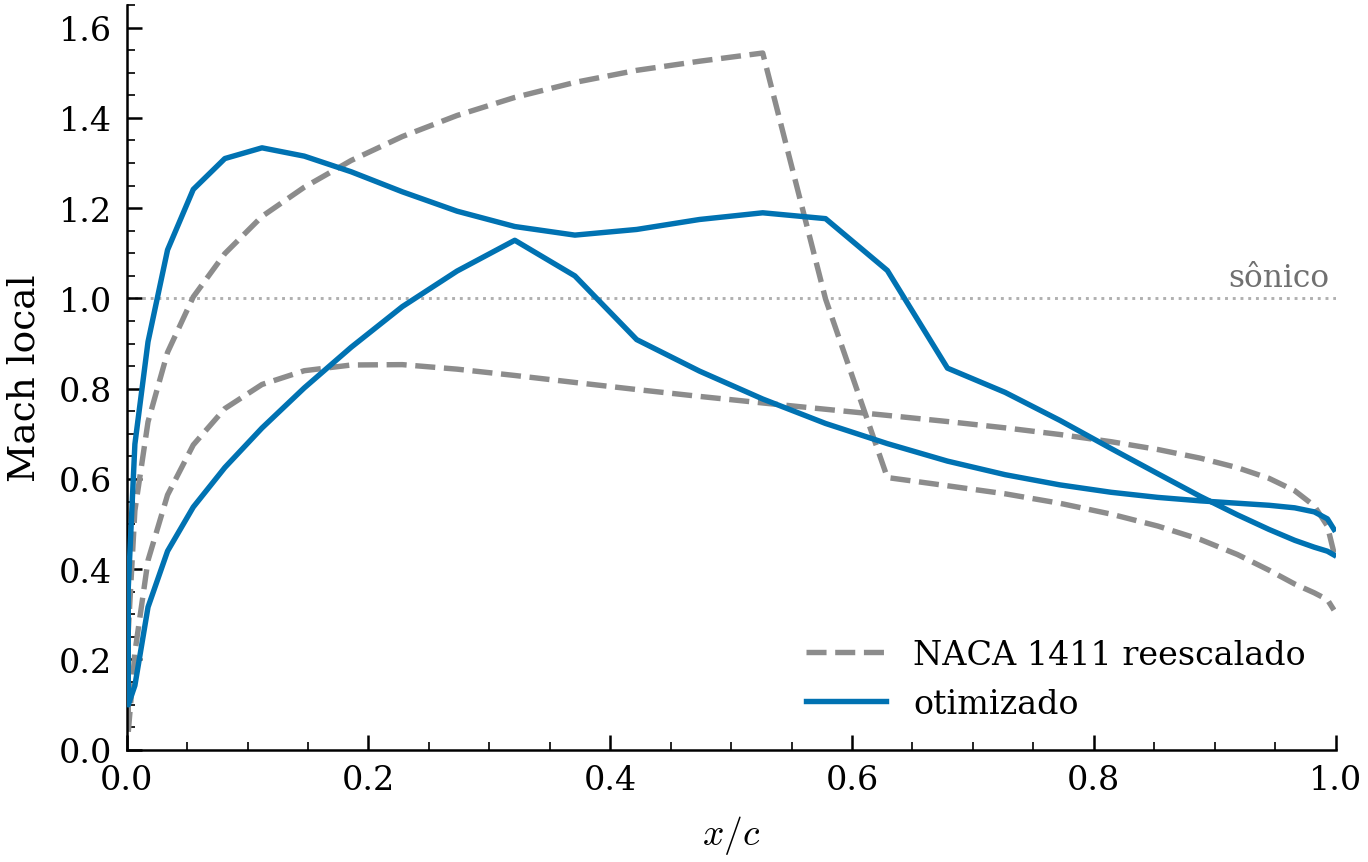
\includegraphics[width=0.8\textwidth]{images/05_transonico/mach.png}
    \caption{Mach local: pico de $1{,}54$ (choque normal) para
    $1{,}33$; platô do otimizado em $1{,}14$--$1{,}19$ com choque
    fraco em $x/c \approx 0{,}62$.}\label{fig:mach_overlay}
\end{figure}

A estratégia do otimizador tem três partes. O NACA acelera o extradorso
até $M \approx 1{,}5$ e paga num único choque normal forte. O otimizado
achata o extradorso dianteiro (arqueamento máximo de $-0{,}015$ em
$x/c = 0{,}25$) e recua a espessura máxima para $x/c = 0{,}364$, o que
segura o platô supersônico em $M \approx 1{,}15$--$1{,}2$ até um choque
fraco em $x/c \approx 0{,}62$. A sustentação perdida na frente volta
pelo carregamento traseiro, com $A_{l4}$ no batente $-0{,}05$. É o
desenho supercrítico clássico. O preço é o $c_m$ mais negativo
($-0{,}068$ para $-0{,}097$), discutido na Seção~7.
